\begin{figure}
    \centering
    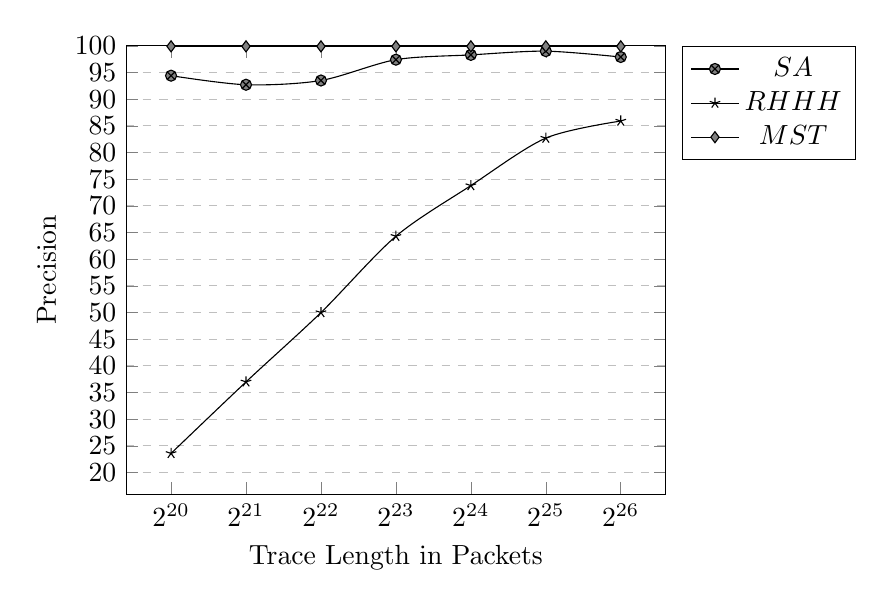
\begin{tikzpicture}
        \begin{axis}[
        xlabel={Trace Length in Packets},
        ylabel={Precision},
        xtick=data,
        xticklabels={$2^{20}$, $2^{21}$, $2^{22}$, $2^{23}$, $2^{24}$, $2^{25}$, $2^{26}$},
        ytick={0,5,10,15,20,25,30,35,40,45,50,55,60,65,70,75,80,85,90,95,100},
        % legend pos=south east,
        % legend columns=2,
        ymajorgrids=true,
        ymax=100,
        grid style=dashed,
        legend style ={ at={(1.03,1)}, 
        anchor=north west, draw=black, 
        fill=white,align=left},
        cycle list name=black white,
        smooth
        ]
            \addplot
            coordinates {
                (1,94.4)(2,92.7)(3,93.5)(4,97.4)(5,98.3)(6,99.0)(7,97.9)
            };
            \addlegendentry{$SA$};
            \addplot
            coordinates {
                (1,23.6)(2,37.0)(3,50.0)(4,64.3)(5,73.8)(6,82.7)(7,85.9)
            };
            \addlegendentry{$RHHH$};
            \pgfplotsset{cycle list shift=2}
            \addplot
            coordinates {
                (1,99.9)(2,99.9)(3,99.9)(4,99.9)(5,99.9)(6,99.9)(7,99.9)
            };
            \addlegendentry{$MST$};
        \end{axis}
    \end{tikzpicture}
    \caption{The precision of ~\ref{algo:sa} Algorithm compared to ``MST" and ``RHHH" on CAIDA'16 trace, for $\phi=0.01, \epsilon=0.001, C=\frac{H}{\epsilon}=\frac{32}{0.001}=32k$ on single bit IP source hierarchy for various lengths the trace.}
    \label{fig:trace_length_precision}
\end{figure}


